% ============================================================
% VEGA SENTINEL - Hackathon Project Report
% EMBRIX'26 - VEGATHON 2026 | Track 2: Edge AI & TinyML Challenge
% Team: Abnormal Detectors - SSNCE
%
% Overleaf: compile with pdfLaTeX.
% Images: the \reportimage command compiles even if an image file is
% missing (it shows a placeholder box). To include real images, upload
% files with the exact names referenced below.
% ============================================================

\documentclass[11pt]{article}

\usepackage[a4paper, margin=2.2cm]{geometry}
\usepackage{graphicx}
\usepackage{booktabs}
\usepackage{tabularx}
\usepackage{listings}
\usepackage{xcolor}
\usepackage{enumitem}
\usepackage{caption}
\usepackage{tikz}
\usetikzlibrary{positioning, arrows.meta, shapes.geometric}
\usepackage[colorlinks=true, linkcolor=blue!60!black, urlcolor=blue]{hyperref}

% ---------- listings style ----------
\lstdefinestyle{cppstyle}{
  language=C++,
  basicstyle=\ttfamily\scriptsize,
  keywordstyle=\color{blue!70!black},
  commentstyle=\color{green!45!black},
  stringstyle=\color{red!60!black},
  breaklines=true,
  frame=single,
  framesep=4pt,
  showstringspaces=false,
  tabsize=4
}

% ---------- caption setup ----------
\captionsetup{font=small, labelfont=bf}

% ---------- image helper: compiles with or without the image ----------
\newcommand{\reportimage}[2]{%
  \begin{center}
    \IfFileExists{#1}{%
      \includegraphics[width=#2\textwidth]{#1}%
    }{%
      \fbox{\parbox[c][4.5cm][c]{#2\textwidth}{\centering
        \textbf{[ INSERT IMAGE HERE ]}\\[4pt]
        Upload the file \texttt{\detokenize{#1}} to this Overleaf project,\\
        or replace this box with \texttt{\textbackslash includegraphics}.}}%
    }%
  \end{center}
}

% ---------- shorthand ----------
\newcommand{\celsius}{\,$^\circ$C}

\begin{document}

% ============================================================
% TITLE PAGE
% ============================================================
\begin{titlepage}
  \centering
  \vspace*{2cm}
  {\Huge\bfseries VEGA SENTINEL\par}
  \vspace{0.5cm}
  {\LARGE AI-Powered Predictive Anomaly Detection at the Edge\par}
  \vspace{1.2cm}
  {\large Edge-AI Multi-Sensor Anomaly Detection for Enclosed Space Safety\par}
  \vspace{1.5cm}
  {\large\bfseries Team Abnormal Detectors\par}
  \vspace{0.3cm}
  {\large EMBRIX'26 -- VEGATHON 2026\par}
  {\large Track 2 -- Edge AI \& TinyML Challenge\par}
  \vspace{0.8cm}
  {\large Sri Sivasubramaniya Nadar College of Engineering (SSNCE)\par}
  \vfill
  {\large September 2026\par}
  \vspace{1cm}
\end{titlepage}

% ============================================================
\section{Team Members}
% ============================================================

\begin{table}[h]
\centering
\begin{tabular}{cl}
\toprule
\textbf{Name} & \textbf{Role / Contribution} \\
\midrule
Hariharan S   & Project Lead \\
Sriarthan R   & Hardware Lead \\
Maheshwaran T & Software Lead \\
Tamilarasan S & Testing \\
\bottomrule
\end{tabular}
\end{table}

% ============================================================
\section{Abstract}
% ============================================================
VEGA SENTINEL is an AI-powered predictive anomaly detection system that
analyses real-time multi-sensor data entirely at the edge. The prototype
combines a VEGA ARIES v2.0 RISC-V controller with three environmental
sensors (MQ-2 gas/smoke sensor, DHT22 temperature/humidity sensor, and an
IR flame sensor) and a buzzer alert mechanism. A sliding-window
feature pipeline feeds a trained logistic-regression model that executes
directly on the microcontroller in C++, so no cloud communication, data
transfer, or network round-trip is required for a safety response.

\textbf{Project-specific measured results:}
\begin{itemize}[nosep]
  \item Trained model (Model A) executed on the ARIES v2.0 board:
        reference normal window scored
        $p = 0.018949 \rightarrow$ NORMAL, reference abnormal window
        $p = 0.992752 \rightarrow$ ABNORMAL (both correct).
  \item 7-fold stratified cross-validation accuracy on the collected
        dataset: \textbf{0.9446} (development result; random window
        split, leakage caveats apply).
  \item Leakage-aware leave-one-trial-out validation:
        \textbf{0.7449} --- the honest development figure.
  \item Real controlled flame trial: flame sensor detected the flame;
        one live window scored $p \approx 0.34 <$ 0.5 (missed detection)
        --- documented honestly; dataset expansion and retraining are
        in progress. Real-world accuracy is \emph{not yet validated}.
\end{itemize}

% ============================================================
\section{Introduction}
% ============================================================
Enclosed spaces --- laboratories, server rooms, storage areas, workshops
and hostel rooms --- can develop dangerous conditions from smoke,
gas-related events, abnormal temperature/humidity drift, or fire.
Conventional threshold alarms examine one sensor against a fixed limit
and ignore how conditions change \emph{together over time}, while
cloud-based smart systems depend on connectivity, add latency and cost,
and stop working when the network drops --- unacceptable for a safety
function.

VEGA SENTINEL brings predictive anomaly detection closer to the
monitored space itself: sensor information is collected, cleaned,
analysed by a lightweight edge model, classified, and used to trigger an
immediate local alert. The decision function is \emph{learned from
collected data}, not a set of hand-tuned thresholds, and runs entirely
on the indigenous VEGA RISC-V platform.

% ============================================================
\section{Problem Statement}
% ============================================================
\textbf{Predictive Analytics \& Anomaly Detection.}
The project aims to detect abnormal conditions from multi-sensor
temporal patterns and provide early warning of possible hazardous
conditions in enclosed spaces, using Edge AI / TinyML on a low-cost
edge device (VEGA ARIES v2.0), with no dependence on cloud
connectivity.

% ============================================================
\section{Objectives}
% ============================================================
\begin{enumerate}[nosep]
  \item Monitor relevant environmental conditions in real time
        (temperature, humidity, gas/smoke-related sensor response,
        flame presence).
  \item Preprocess sensor readings with a validity gate and sliding
        windows to reduce noise and obtain useful temporal features.
  \item Use a lightweight edge-based AI/TinyML approach (trained
        logistic-regression classifier executing in C++) for pattern
        analysis.
  \item Classify operating conditions as Normal or Abnormal
        (data collection additionally used a Warning label).
  \item Analyse changing temporal patterns (window dynamics and
        multi-window persistence) to support early indication of a
        developing abnormal condition.
  \item Trigger an audible alert so preventive action can be taken,
        with temporal confirmation to suppress single-window noise.
\end{enumerate}

% ============================================================
\section{Proposed System}
% ============================================================
VEGA SENTINEL combines a VEGA ARIES v2.0 controller with multiple
sensors and an alert mechanism. The prototype components are an IR
flame sensor, a DHT22 temperature and humidity sensor, an MQ-2 gas
sensor, and a buzzer driven through a 2N2222 transistor stage. The
overall concept is to process sensor information at the edge and
generate an immediate local response when abnormal behaviour is
detected.

\begin{figure}[ht]
\centering
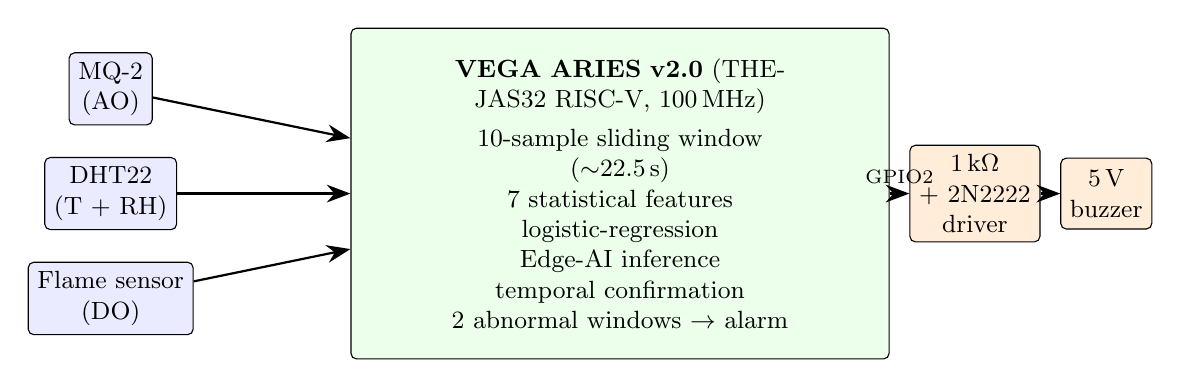
\begin{tikzpicture}[
  box/.style={draw, rounded corners=2pt, align=center, font=\small, minimum height=9mm},
  sens/.style={box, fill=blue!8},
  proc/.style={box, fill=green!8},
  act/.style={box, fill=orange!15},
  arrow/.style={-{Stealth[length=3mm]}, thick}]

  \node[sens] (mq2)   {MQ-2\\(AO)};
  \node[sens, below=4mm of mq2]  (dht)   {DHT22\\(T + RH)};
  \node[sens, below=4mm of dht]   (flame) {Flame sensor\\(DO)};

  \node[proc, right=2.2cm of dht, minimum height=4.2cm, text width=6.6cm]
    (aries) {\textbf{VEGA ARIES v2.0} (THEJAS32 RISC-V, 100\,MHz)\\[3pt]
      10-sample sliding window\\($\sim$22.5\,s)\\
      7 statistical features\\
      logistic-regression\\Edge-AI inference\\
      temporal confirmation\\
      2 abnormal windows $\rightarrow$ alarm};

  \node[act, right=2.5mm of aries] (drv) {1\,k$\Omega$\\+ 2N2222\\driver};
  \node[act, right=2.5mm of drv]  (bz)  {5\,V\\buzzer};

  \draw[arrow] (mq2)   -- (aries);
  \draw[arrow] (dht)   -- (aries);
  \draw[arrow] (flame) -- (aries);
  \draw[arrow] (aries) -- node[above, font=\scriptsize, draw=none]{GPIO2} (drv);
  \draw[arrow] (drv)   -- (bz);
\end{tikzpicture}
\caption{Proposed system block diagram.}
\end{figure}

% ============================================================
\section{System Architecture}
% ============================================================
The workflow follows the pattern:

\begin{center}
\fbox{SENSE} $\rightarrow$ \fbox{CLEAN} $\rightarrow$ \fbox{THINK}
$\rightarrow$ \fbox{DETECT} $\rightarrow$ \fbox{PREDICT}
$\rightarrow$ \fbox{ACT}
\end{center}

\begin{description}
  \item[SENSE] Collect live sensor data every 2500\,ms: DHT22
    (bit-banged 1-wire driver, checksum-verified), MQ-2 analog output
    through a 2\,$\times$\,2.2\,k$\Omega$ divider into A0 (raw ADC
    counts), flame sensor digital output (active-LOW) on GPIO1.
  \item[CLEAN] Validate every sample before use: DHT22 checksum and
    plausibility range checks. Invalid samples are discarded; the
    sliding window is \emph{not} shifted and the alarm state is
    preserved. Valid samples update a 10-sample window
    ($\sim$22.5\,s of history) from which 7 statistical features are
    computed.
  \item[THINK] A lightweight trained model (logistic regression with
    embedded standardisation constants, implemented in plain C++)
    converts the 7 features into an abnormality probability on the
    microcontroller itself.
  \item[DETECT] Each window is classified NORMAL or ABNORMAL against
    a fixed 0.5 threshold (never tuned to force a demonstration).
  \item[PREDICT] Temporal confirmation analyses the \emph{sequence} of
    AI decisions: 2 consecutive abnormal windows indicate a developing
    condition and arm the alarm; 3 consecutive normal windows are
    required to clear it.
  \item[ACT] GPIO2 switches the buzzer through a 1\,k$\Omega$ base
    resistor and a 2N2222 transistor from an external 5\,V rail, so
    the 12\,mA-limited GPIO never drives the buzzer directly.
\end{description}

% ============================================================
\section{Hardware Components}
% ============================================================

\begin{table}[h]
\centering
\begin{tabularx}{\textwidth}{c l c X}
\toprule
\textbf{S.No} & \textbf{Component} & \textbf{Qty} & \textbf{Key specification / role} \\
\midrule
1 & VEGA ARIES v2.0 board & 1 & THEJAS32/VEGA ET1031 RISC-V @ 100\,MHz, 256\,KB SRAM, 2\,MB flash, 3.3\,V I/O, 4 analog inputs (ADS1015) \\
2 & IR Flame Sensor module & 1 & 3-pin, 3.3\,V, digital DO, active-LOW \\
3 & DHT22 sensor & 1 & Temperature $+$ humidity, 3.3\,V, 1-wire protocol \\
4 & MQ-2 gas sensor module & 1 & 5\,V, analog AO output (gas/smoke-related response) \\
5 & Buzzer (5\,V active) & 1 & Audible alarm, external 5\,V supply \\
6 & 2N2222 transistor & 1 & Buzzer switching driver \\
7 & Resistor 1\,k$\Omega$ & 1 & 2N2222 base current limit \\
8 & Resistor 2.2\,k$\Omega$ & 2 & MQ-2 analog voltage divider \\
\bottomrule
\end{tabularx}
\end{table}

\reportimage{photo_components.jpg}{0.75}

% ============================================================
\section{Function of Components}
% ============================================================
\begin{itemize}[nosep]
  \item \textbf{VEGA ARIES v2.0:} main edge-computing/controller
    board; performs acquisition, windowing, feature extraction, AI
    inference, confirmation logic and alarm control.
  \item \textbf{IR Flame Sensor:} senses the presence of flame
    (experimentally verified active-LOW output).
  \item \textbf{DHT22:} measures temperature and relative humidity.
  \item \textbf{MQ-2 Gas Sensor:} gas/smoke-related sensing; its raw
    analog response is used as an uncalibrated sensor signal (no ppm
    claims).
  \item \textbf{Buzzer + 2N2222 + 1\,k$\Omega$:} audible alert stage;
    the transistor driver keeps the buzzer current off the
    12\,mA-limited GPIO.
  \item \textbf{2\,$\times$\,2.2\,k$\Omega$ divider:} halves the MQ-2
    module's 5\,V analog output so it stays within the safe input
    range of the ARIES analog input.
\end{itemize}

% ============================================================
\section{Sensor Data Acquisition}
% ============================================================
The prototype uses the following sensor inputs, sampled on a common
cadence:

\begin{itemize}[nosep]
  \item IR flame detection (binary, active-LOW).
  \item Temperature and humidity from DHT22 (checksum-verified,
    bit-banged driver).
  \item Gas/smoke-related raw analog reading from MQ-2 via the
    divider on A0.
  \item \textbf{Sampling interval: 2500\,ms} (all sensors; bounded by
    the DHT22 requirement of $\geq$2\,s between reads).
\end{itemize}

\textbf{Sensor operating ranges / calibration details:}
\begin{itemize}[nosep]
  \item DHT22: 0--100\,\%RH, $-40$ to $+80$\celsius{} (observed in
    sessions: 27.8--28.8\celsius{} and 68.7--80.3\,\%RH).
  \item MQ-2: \textbf{raw ADC counts 0--2047} on this board (onboard
    ADS1015, single-ended, measured effective range; observed clean-air
    baseline $\sim$101--259 counts). The MQ-2 is \emph{not} a
    calibrated gas-concentration instrument; values are raw sensor
    responses, not ppm.
  \item Flame sensor: digital, active-LOW (LOW = flame detected),
    verified experimentally on our module.
\end{itemize}

% ============================================================
\section{Data Preprocessing}
% ============================================================
The system filters noisy or inconsistent sensor readings and converts
raw readings into useful inputs for the edge model.

\textbf{Actual filtering method:} every acquisition is read into
temporary variables first and validated (DHT22 checksum +
plausibility range, MQ-2 ADC range). Only a \emph{valid} sample updates
the sliding window. On failure the sample is discarded, the window is
not shifted, no inference runs, and the alarm state is preserved ---
stale values are never used as new measurements. (This fixed an earlier
firmware issue where the window was shifted before validation.)

\textbf{Features calculated} (over a 10-sample window,
$\sim$22.5\,s):

\begin{table}[h]
\centering
\begin{tabular}{cl}
\toprule
\textbf{Feature} & \textbf{Definition} \\
\midrule
\texttt{humidity\_mean}  & mean relative humidity in window \\
\texttt{temp\_mean}      & mean temperature in window \\
\texttt{mq2\_range}      & max $-$ min of MQ-2 raw ADC in window \\
\texttt{mq2\_delta}      & last $-$ first MQ-2 value in window (trend) \\
\texttt{mq2\_std}        & sample std ($n-1$) of MQ-2 in window \\
\texttt{humidity\_std}   & sample std ($n-1$) of humidity \\
\texttt{flame\_fraction} & fraction of window samples with flame detected \\
\bottomrule
\end{tabular}
\caption{The 7 model input features.}
\end{table}

The same window/feature logic is used offline for training-data
generation and on-device at runtime, so the model's learned feature
distribution matches deployment.

% ============================================================
\section{Edge AI / TinyML Implementation}
% ============================================================

\begin{table}[h]
\centering
\begin{tabularx}{\textwidth}{l X}
\toprule
\textbf{Model / algorithm} & Logistic regression (sigmoid probability)
  with embedded standardisation (Model A). Trained, not hand-tuned
  thresholds. Inference is direct C/C++ arithmetic on the board; no
  TensorFlow Lite Micro / Edge Impulse (not verified on ARIES v2.0). \\
\textbf{Dataset} & 5 collection sessions ($\sim$45\,min total,
  1085 valid samples) $\rightarrow$ 107 windows:
  \textbf{100 normal / 7 abnormal}. A window is abnormal if it
  contains any \texttt{critical} event label. \\
\textbf{Input features} & 7 (table above); fixed order enforced across
  training script, exported header, and firmware. \\
\textbf{Output classes} & 2 deployed: NORMAL / ABNORMAL
  (data collection additionally used normal/warning/critical labels). \\
\textbf{Training platform} & Python 3 + scikit-learn
  (\texttt{StandardScaler} + \texttt{LogisticRegression},
  \texttt{class\_weight="balanced"}, \texttt{random\_state}=42);
  constants exported automatically to a C++ header. \\
\textbf{Accuracy} & 7-fold stratified CV: \textbf{0.9446} (development
  estimate; random window split, overlap leakage possible).
  Leave-one-trial-out: \textbf{0.7449}. On-board reference windows:
  $p=0.018949 \rightarrow$ NORMAL, $p=0.992752 \rightarrow$ ABNORMAL
  (math execution verified on ARIES). Real-world accuracy
  \emph{not yet validated}. \\
\textbf{Model size} & 22 constants (7 means, 7 scales, 7 coefficients,
  intercept) $\approx$ 88 bytes of flash; the entire inference routine
  including feature code is well under 1\,KB. \\
\textbf{Inference time} & Not yet formally benchmarked. The computation
  is 7 multiply--adds and one sigmoid per window step
  ($\ll$1\,ms at 100\,MHz, estimated). \\
\bottomrule
\end{tabularx}
\caption{Edge-AI implementation summary (all values measured or
reproducible from the repository; nothing fabricated).}
\end{table}

% ============================================================
\section{Anomaly Detection and Prediction}
% ============================================================
The system classifies the operating condition and examines changing
patterns to estimate a possibly developing abnormal condition.

\begin{table}[h]
\centering
\begin{tabularx}{\textwidth}{l >{\raggedright\arraybackslash}X >{\raggedright\arraybackslash}X}
\toprule
\textbf{State} & \textbf{Detection condition} & \textbf{System response} \\
\midrule
Normal & Window probability $p < 0.5$ &
  No alarm; buzzer OFF; CSV logging continues. \\
Warning & Mild deviation label used during data collection (not a
  deployed classifier class); a single abnormal window in isolation &
  Logged for review; deliberately no alarm yet --- the temporal
  confirmation layer suppresses single-window noise. \\
Anomaly & $p \geq 0.5$ on \textbf{2 consecutive windows} &
  Buzzer ON via 2N2222 driver; cleared only after \textbf{3
  consecutive normal windows}. \\
\bottomrule
\end{tabularx}
\caption{Detection states and responses.}
\end{table}

\textbf{Prediction criteria / failure indicators:} the window dynamics
(\texttt{mq2\_range}, \texttt{mq2\_delta}, \texttt{mq2\_std},
\texttt{humidity\_std}) capture a condition that is \emph{developing}
across $\sim$22.5\,s, and the multi-window persistence counters
require the condition to persist across $\sim$5\,s of consecutive
abnormal decisions --- providing early warning of a developing
hazard rather than reacting to a single noisy sample.

% ============================================================
\section{Alert Mechanism}
% ============================================================
When an abnormal condition is confirmed, the system triggers an
immediate local alert.

\begin{itemize}[nosep]
  \item \textbf{Buzzer activation condition:} 2 consecutive AI windows
    classified ABNORMAL ($p \geq 0.5$). The alarm clears after 3
    consecutive normal windows.
  \item \textbf{Other alert mechanism:} the firmware streams a CSV
    telemetry line and an explicit AI decision line
    (\texttt{AI,p=\dots,status=NORMAL/ABNORMAL}) over USB serial at
    115200 baud for live monitoring and dataset logging.
\end{itemize}

% ============================================================
\section{Circuit and Wiring}
% ============================================================

\begin{table}[h]
\centering
\begin{tabularx}{\textwidth}{l l l X}
\toprule
\textbf{Component} & \textbf{VCC} & \textbf{GND} & \textbf{Signal / output pin} \\
\midrule
DHT22 & ARIES 3.3\,V & ARIES GND &
  DATA $\rightarrow$ GPIO0 (module pull-up to 3.3\,V; the VEGA core
  provides no internal pull-up) \\
IR Flame Sensor & ARIES 3.3\,V & ARIES GND &
  DO $\rightarrow$ GPIO1 (active-LOW: LOW = flame detected) \\
MQ-2 Gas Sensor & 5\,V & GND (common) &
  AO $\rightarrow$ 2\,$\times$\,2.2\,k$\Omega$ divider $\rightarrow$ A0
  (halves the 5\,V output; DO unused) \\
Buzzer & External 5\,V ($+$) & via driver to common GND &
  GPIO2 $\rightarrow$ 1\,k$\Omega$ $\rightarrow$ 2N2222 base;
  emitter $\rightarrow$ GND; collector $\rightarrow$ buzzer $(-)$ \\
\bottomrule
\end{tabularx}
\caption{Verified wiring summary.}
\end{table}

\textbf{Design rules encoded in the circuit:} (1) no GPIO ever drives
the buzzer directly --- the 12\,mA per-I/O limit forbids it, so the
2N2222 stage does the switching; (2) the 5\,V MQ-2 output never
reaches an analog pin directly --- the divider keeps A0 at or below
2.5\,V; (3) a common ground across the board, all sensors and the
buzzer supply is mandatory.

\reportimage{schematic_circuit.jpg}{0.8}

% ============================================================
\section{Software Implementation}
% ============================================================
The software continuously acquires sensor information, validates it,
performs the required preprocessing, analyses the resulting features,
determines the current condition, and activates the alert mechanism
when required.

\begin{figure}[ht]
\centering
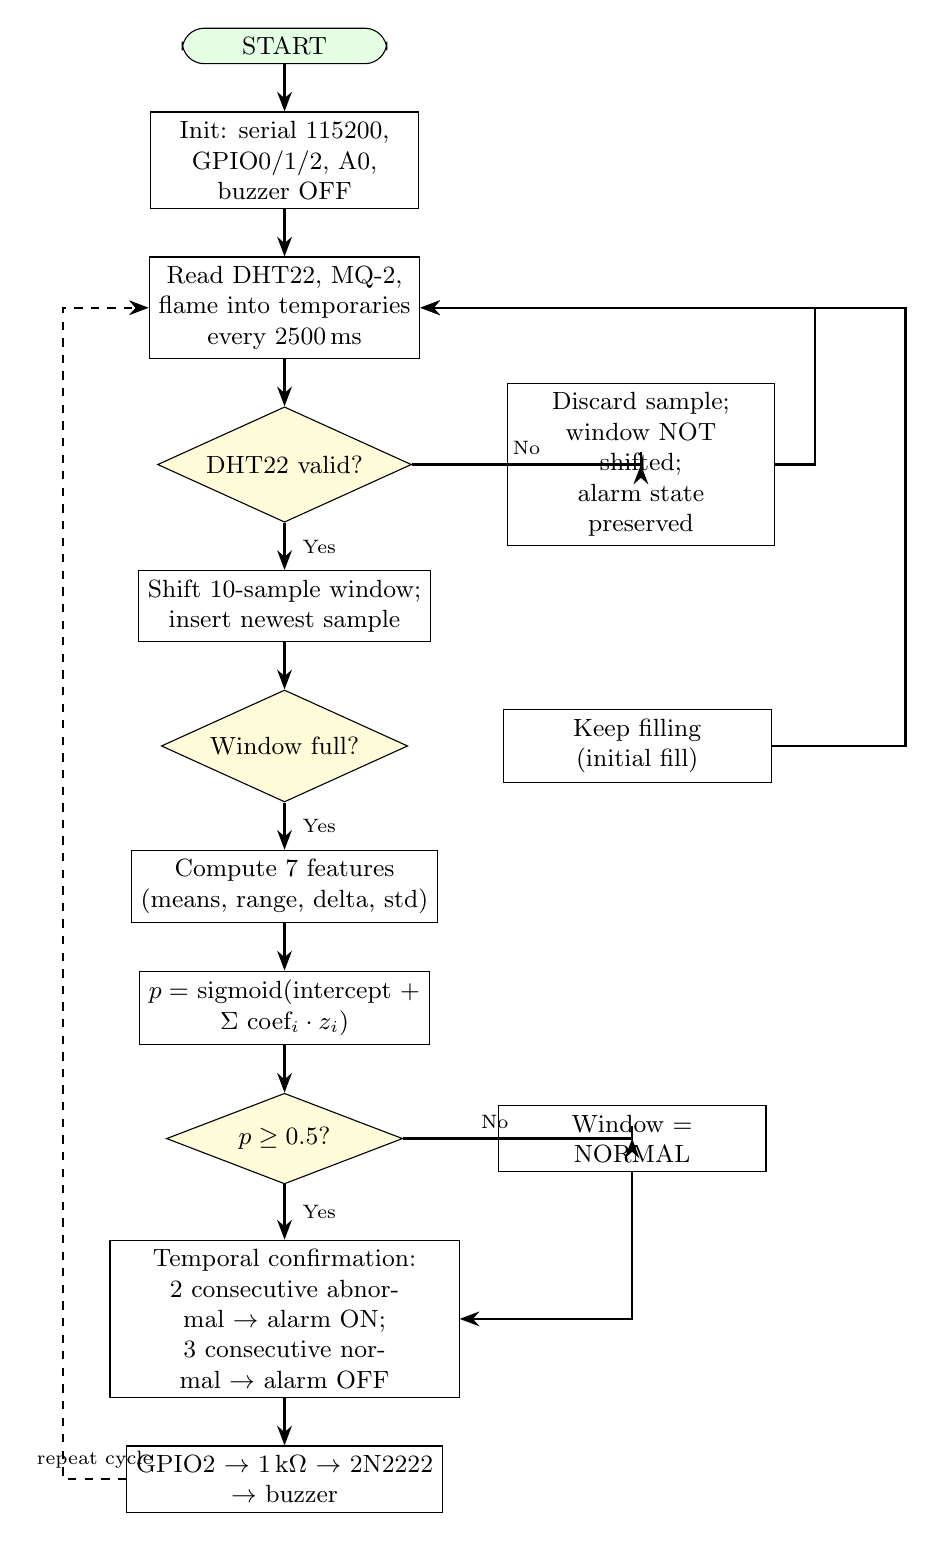
\begin{tikzpicture}[
  node distance=6mm and 10mm,
  startstop/.style={draw, rounded corners=8pt, fill=green!10, font=\small, align=center, minimum width=26mm},
  proc/.style={draw, font=\small, align=center, minimum width=34mm},
  dec/.style={draw, diamond, aspect=2.2, fill=yellow!15, font=\small, align=center, minimum width=30mm},
  arrow/.style={-{Stealth[length=2.5mm]}, thick},
  lbl/.style={font=\scriptsize, draw=none}]

  \node[startstop] (start) {START};
  \node[proc, below=of start] (init) {Init: serial 115200,\\GPIO0/1/2, A0,\\ buzzer OFF};
  \node[proc, below=of init] (read) {Read DHT22, MQ-2,\\flame into temporaries\\every 2500\,ms};
  \node[dec, below=of read] (valid) {DHT22 valid?};
  \node[proc, right=12mm of valid, text width=28mm] (discard) {Discard sample;\\window NOT shifted;\\alarm state preserved};
  \node[proc, below=of valid] (shift) {Shift 10-sample window;\\insert newest sample};
  \node[dec, below=of shift] (full) {Window full?};
  \node[proc, right=12mm of full, text width=28mm] (wait1) {Keep filling\\(initial fill)};
  \node[proc, below=of full] (feat) {Compute 7 features\\(means, range, delta, std)};
  \node[proc, below=of feat] (infer) {$p = $ sigmoid(intercept +\\$\Sigma$ coef$_i \cdot z_i$)};
  \node[dec, below=of infer] (th) {$p \geq 0.5$?};
  \node[proc, below=7mm of th, text width=42mm] (conf) {Temporal confirmation:\\2 consecutive abnormal $\rightarrow$ alarm ON;\\3 consecutive normal $\rightarrow$ alarm OFF};
  \node[proc, below=of conf] (buz) {GPIO2 $\rightarrow$ 1\,k$\Omega$ $\rightarrow$ 2N2222\\$\rightarrow$ buzzer};
  \node[proc, right=12mm of th, text width=24mm] (norm) {Window =\\NORMAL};

  \draw[arrow] (start) -- (init);
  \draw[arrow] (init) -- (read);
  \draw[arrow] (read) -- (valid);
  \draw[arrow] (valid) -| node[lbl, above, pos=0.25]{No} (discard);
  \draw[arrow] (discard.east) -- ++(5mm,0) |- (read.east);
  \draw[arrow] (valid) -- node[lbl, right=1mm]{Yes} (shift);
  \draw[arrow] (shift) -- (full);
  \draw[arrow] (wait1.east) -- ++(17mm,0) |- (read.east);
  \draw[arrow] (full) -- node[lbl, right=1mm]{Yes} (feat);
  \draw[arrow] (feat) -- (infer);
  \draw[arrow] (infer) -- (th);
  \draw[arrow] (th) -| node[lbl, above, pos=0.2]{No} (norm);
  \draw[arrow] (norm) |- (conf);
  \draw[arrow] (th) -- node[lbl, right=1mm]{Yes} (conf);
  \draw[arrow] (conf) -- (buz);
  \draw[arrow, dashed] (buz.west) -- node[lbl, above]{repeat cycle} ++(-8mm,0) |- (read.west);
\end{tikzpicture}
\caption{Firmware flowchart (one monitoring cycle).}
\end{figure}

% ============================================================
\section{Algorithm / Program Flow}
% ============================================================
\begin{enumerate}[nosep]
  \item Initialise the VEGA ARIES v2.0 board: serial (115200 baud),
    GPIO0 (DHT22), GPIO1 (flame, input), GPIO2 (buzzer, output,
    OFF), A0 (MQ-2).
  \item Every 2500\,ms, read all sensors into temporary variables.
  \item Validate the DHT22 sample (checksum + plausibility). If
    invalid: discard the sample, keep the window and alarm state
    unchanged, and wait for the next cycle.
  \item On a valid sample: shift the 10-sample window and insert the
    newest values.
  \item When the window is full: compute the 7 features and standardise
    them with the embedded scaler constants.
  \item Run the logistic-regression model (dot product + sigmoid) and
    classify the window NORMAL ($p<0.5$) or ABNORMAL ($p \geq 0.5$).
  \item Update the temporal confirmation counters: 2 consecutive
    abnormal windows arm the alarm; 3 consecutive normal windows
    clear it.
  \item Drive the buzzer accordingly through the 2N2222 stage and emit
    the CSV/decision telemetry lines.
  \item Repeat the monitoring cycle.
\end{enumerate}

% ============================================================
\section{Code}
% ============================================================
The complete, tested source code is in the project repository:
\begin{center}
  \url{https://github.com/hariharanboss/VEGA-Sentinel}
\end{center}
(firmware under \texttt{firmware/}, reproducible ML pipeline under
\texttt{ml/}, datasets under \texttt{dataset/}). The core on-device
inference and confirmation logic, verbatim from the final firmware:

\begin{lstlisting}[style=cppstyle]
// Model A inference: standardise -> linear score -> sigmoid
float modelPredict(float features[])
{
    float score = MODEL_INTERCEPT;
    for (int i = 0; i < MODEL_NUM_FEATURES; i++)
    {
        float standardized =
            (features[i] - MODEL_MEANS[i]) / MODEL_SCALES[i];
        score += MODEL_COEFFS[i] * standardized;
    }
    if (score > 30.0f)  return 1.0f;   // numerically safe
    if (score < -30.0f) return 0.0f;  // sigmoid clamps
    return 1.0f / (1.0f + expf(-score));
}

// Temporal confirmation: 2 consecutive abnormal -> alarm ON,
// 3 consecutive normal -> alarm OFF (buzzer via 2N2222)
void processWindowClassification(bool abnormal)
{
    if (abnormal) {
        consecutiveAbnormal++; consecutiveNormal = 0;
        if (consecutiveAbnormal >= 2 && !alarmActive) {
            alarmActive = true; }        // buzzer ON
    } else {
        consecutiveNormal++; consecutiveAbnormal = 0;
        if (consecutiveNormal >= 3 && alarmActive) {
            alarmActive = false; }       // buzzer OFF
    }
    digitalWrite(PIN_BUZZER, alarmActive ? HIGH : LOW);
}
\end{lstlisting}

% ============================================================
\section{Required Libraries}
% ============================================================
\begin{itemize}[nosep]
  \item \textbf{Firmware:} no external libraries. The VEGA Arduino
    core (C-DAC v1.1.2) provides the Arduino API used
    (\texttt{Serial}, \texttt{pinMode}, \texttt{digitalRead},
    \texttt{analogRead}, \texttt{micros}); the DHT22 driver is
    self-contained bit-banged code and the model is plain C/C++
    arithmetic.
  \item \textbf{PC pipeline (training/data tools):}
    \texttt{pandas}, \texttt{numpy}, \texttt{scikit-learn},
    \texttt{matplotlib}, \texttt{pyserial}.
\end{itemize}

% ============================================================
\section{Code Explanation}
% ============================================================
\begin{description}
  \item[Initialization:] serial at 115200 baud; GPIO0/1 configured;
    GPIO2 set OUTPUT and LOW (buzzer off); analog input A0.
  \item[Sensor reading:] DHT22 via the bit-banged one-wire driver with
    checksum verification ($\geq$2\,s between reads); MQ-2 as a single
    \texttt{analogRead} (raw counts); flame via
    \texttt{digitalRead} with active-LOW normalisation.
  \item[Data preprocessing:] validity gate before any state change;
    fixed-size 10-sample window (static arrays, no dynamic
    allocation); 7 features with sample standard deviation ($n-1$),
    matching the offline training computation exactly.
  \item[AI/TinyML inference:] embedded scaler constants
    (mean/scale per feature) + logistic-regression coefficients +
    sigmoid, all generated automatically from the training pipeline
    into \texttt{model.h}.
  \item[Classification:] per-window binary decision against the fixed
    0.5 threshold.
  \item[Prediction:] multi-window persistence analysis (consecutive
    abnormal/normal counters) that turns per-window decisions into a
    stable early-warning state.
  \item[Buzzer control:] GPIO2 drives only the 2N2222 base through
    1\,k$\Omega$ ($\approx$2.6\,mA); the buzzer itself is switched
    from the external 5\,V rail.
\end{description}

% ============================================================
\section{Testing and Results}
% ============================================================
Testing verified sensor readings, classification behaviour, and alert
response under normal and selected \emph{safe, supervised} abnormal
conditions.

\begin{table}[h]
\centering
\scriptsize
\begin{tabularx}{\textwidth}{c X X X}
\toprule
\textbf{Test} & \textbf{Condition / expected} & \textbf{Actual result} & \textbf{Remarks} \\
\midrule
1 & Board bring-up: serial prints at 115200 & Pass & IDE + VEGA core (ARIES v2) verified \\
2 & Onboard ADC (ADS1015) stability & Pass & Stable counts; effective single-ended range 0--2047 \\
3 & DHT22 bit-banged read & Pass & Temperature/humidity track room; checksum errors rare \\
4 & MQ-2 via divider & Pass & Clean-air baseline $\sim$101--259 counts; responds to safe stimulus; warm-up noted \\
5 & Flame sensor polarity & Pass & Active-LOW verified; 5 flame-positive rows recorded in committed trials \\
6 & Buzzer driver (2N2222) & Pass & ON/OFF on GPIO2; GPIO load $\approx$2.6\,mA (within 12\,mA limit) \\
7 & Model A math on ARIES & Pass & $p=0.018949 \rightarrow$ NORMAL; $p=0.992752 \rightarrow$ ABNORMAL (matches PC) \\
8 & Live sliding-window inference & Pass & New AI decision every 2.5\,s after window fill; DHT-failure window preservation verified \\
9 & Controlled flame trial (live) & \textbf{Partial} & Flame detected by sensor; one live window scored $p \approx 0.34 \rightarrow$ NORMAL, buzzer OFF \\
\bottomrule
\end{tabularx}
\caption{Test record (all results actually executed; nothing fabricated).}
\end{table}

\textbf{Measured sensor values:} temperature 27.8--28.8\celsius{},
humidity 68.7--80.3\,\%RH, MQ-2 raw ADC 101--259 counts, flame binary
(active-LOW), across 5 committed sessions on 2026-09-11.

\textbf{Model quality (development, not final):} random-split CV
0.9446; leave-one-trial-out 0.7449; a real flame trial produced one
missed detection (test 9) --- root cause is the small dataset (7
abnormal windows), not the architecture. The response is more data and
retraining with trial-level validation, \emph{not} a hard-coded
flame-to-buzzer rule and \emph{not} a tuned threshold.

\textbf{Overall observed result:} the end-to-end pipeline (sensors
$\rightarrow$ windowing $\rightarrow$ on-board AI $\rightarrow$
confirmation $\rightarrow$ alarm) works on hardware. Final real-world
performance is not yet validated; dataset expansion is in progress.

\reportimage{vega_sentinel_mq2_comparison.png}{0.85}
\captionof{figure}{MQ-2 sensor response comparison across sessions.}
\reportimage{vega_sentinel_flame_incident.png}{0.85}
\captionof{figure}{Flame-trial incident analysis.}

% ============================================================
\section{Project Output}
% ============================================================

\reportimage{photo_output_1.jpg}{0.8}
\captionof{figure}{VEGA SENTINEL output / test photograph 1.}

\reportimage{photo_output_2.jpg}{0.8}
\captionof{figure}{VEGA SENTINEL output / test photograph 2.}

\reportimage{photo_output_3.jpg}{0.8}
\captionof{figure}{VEGA SENTINEL output / test photograph 3.}

% ============================================================
\section{Feasibility and Scalability}
% ============================================================
\textbf{Feasibility.} The system uses low-cost sensors and a
low-cost indigenous controller, making it affordable and easy to
deploy. The model is deliberately tiny (88 bytes of constants,
no framework), so it operates comfortably within the 256\,KB SRAM /
2\,MB flash of the ARIES v2.0, and every result in this report was
produced on the actual hardware.

\textbf{Challenges.} Noisy or inconsistent sensor readings (DHT22
checksum failures, MQ-2 warm-up and baseline drift); different rooms
produce different normal environmental patterns; small datasets
weaken generalization (demonstrated honestly by test 9).

\textbf{Proposed solutions.} A validity gate before window updates
(implemented); deployment-consistent window/feature generation
(implemented); continuous data collection and trial-level validation
to improve and honestly measure accuracy over time (in progress).

\textbf{Scalability.} The architecture extends from one enclosed space
to many using the same edge-AI pattern (each unit learns its own
room's normal profile); additional sensors and anomaly types can be
added by extending the feature set and retraining, without redesigning
the system.

% ============================================================
\section{Impact and Benefits}
% ============================================================
\begin{itemize}[nosep]
  \item \textbf{Early detection:} abnormal temporal patterns are
    flagged while a condition is developing, enabling timely action.
  \item \textbf{Cost reduction:} low-cost hardware, no cloud bills, no
    connectivity requirements.
  \item \textbf{Improved safety:} local, latency-bounded warning for
    enclosed spaces (laboratories, server rooms, storage areas).
  \item \textbf{Energy efficiency:} edge processing removes continuous
    cloud communication.
  \item \textbf{Indian ecosystem:} a complete Edge-AI safety system
    demonstrated on the indigenous VEGA RISC-V platform, suitable for
    institutions and smart infrastructure.
\end{itemize}

% ============================================================
\section{Applications}
% ============================================================
\begin{itemize}[nosep]
  \item Laboratory and workshop environmental safety monitoring.
  \item Server-room / storage-area abnormal-condition warning.
  \item Hostel and residential enclosed-space safety assistance.
  \item Baseline template for predictive maintenance on other
    low-cost edge nodes (same pipeline, different sensors).
\end{itemize}

% ============================================================
\section{Future Scope}
% ============================================================
\begin{itemize}[nosep]
  \item Dataset expansion: 20--30 minutes of fresh normal data plus
    multiple safe, supervised abnormal trials with recovery phases.
  \item Retraining with trial-level (leakage-aware) validation and
    deployment of the improved model via the automated export tool.
  \item On-device benchmarking of inference time and memory usage.
  \item Adaptive baselines for slowly drifting environments
    (humidity/MQ-2 warm-up).
  \item Enclosure/prototype packaging and long-duration soak tests.
  \item Optional long-term logging dashboards on the PC side.
\end{itemize}

% ============================================================
\section{Project Demonstration}
% ============================================================
\textbf{Project video link:} \underline{\hspace{5cm}} \textit{(to be
added)}

\reportimage{video_qr_screenshot.png}{0.45}

% ============================================================
\section{Conclusion}
% ============================================================
VEGA SENTINEL presents an edge-based approach to predictive anomaly
detection by combining multi-sensor monitoring with lightweight
AI/TinyML processing on the indigenous VEGA ARIES v2.0 RISC-V
platform. Its SENSE--CLEAN--THINK--DETECT--PREDICT--ACT workflow
provides early warnings, removes dependence on cloud processing, and
supports safer monitoring of enclosed spaces.

\textbf{Final project results and performance:} the complete pipeline
is physically implemented and working --- trained model executing
on-board with math verified against the PC implementation
($p=0.018949$ / $p=0.992752$ on reference windows), live sliding-window
inference every 2.5\,s, and a hardware-verified alarm stage. Model
quality is a \emph{development result} (CV 0.9446 with leakage
caveats; 0.7449 trial-level), a real flame-trial miss is documented,
and final accuracy claims await the in-progress dataset expansion and
retraining. The system is an honest, reproducible prototype --- not a
certified safety device, and no unmeasured performance is claimed.

% ============================================================
\section{CAD / PCB Design (Optional)}
% ============================================================
No custom PCB has been designed yet; the prototype uses the ARIES
v2.0 development board with point-to-point wiring (see the Circuit
and Wiring section). A dedicated PCB is future work.

% ============================================================
\section{References}
% ============================================================
\begin{enumerate}[nosep]
  \item A. Malhotra \emph{et al.}, ``A Holistic Review of the TinyML
    Stack for Predictive Maintenance,'' \emph{IEEE Access}, vol.~12,
    pp.~184861--184882, Dec.~2024. DOI: 10.1109/ACCESS.2024.3512860.
  \item ``TinyMLEdge: A Workflow for Deploying TinyML Models in
    Industrial Edge Devices,'' 2024 IEEE 22nd Int.\ Conf.\ on
    Industrial Informatics (INDIN), 2024.
    DOI: 10.1109/INDIN58382.2024.10774465.
  \item IEEE --- TinyML \& Predictive Maintenance:
    \url{https://ieeexplore.ieee.org/document/10781407}
  \item IEEE --- TinyMLEdge \& Industrial Edge Devices:
    \url{https://ieeexplore.ieee.org/document/10774465}
  \item IEEE --- Anomaly Detection \& Predictive Maintenance:
    \url{https://ieeexplore.ieee.org/document/10586631}
  \item C-DAC, VEGA ARIES v2.0 product page:
    \url{https://www.cdac.in/index.aspx?id=product_details&productId=ARIESv2.0};
    datasheet:
    \url{https://vegaprocessors.in/files/ARIESv2%200_Datasheet_v2.pdf}
  \item F. Pedregosa \emph{et al.}, ``Scikit-learn: Machine Learning
    in Python,'' \emph{JMLR}, vol.~12, pp.~2825--2830, 2011.
  \item Project repository (code, datasets, results):
    \url{https://github.com/hariharanboss/VEGA-Sentinel}
\end{enumerate}

\end{document}
